% mainfile: ../../main.tex
\chapter{Characterization and improvements of the optical path}\label{ch:setup:optics}
\AutoLettrine{Noise}

\section{Light coupling}\label{sec:setup:optics:coupling}
\Glspl{smf} are a natural choice to transmit laser light which usually consists of a just that, a single mode.
Because the mode profile of \glspl{smf} is very close to the fundamental laser mode, \acrshort{tem}$_{00}$, \emph{Gaussian optics} are required to describe the propagating light.

\begin{enumerate}
    \item Gaussian optics equations \begin{enumerate}
        \item electric field profile
        \item rayleigh length
        \item beam divergence \& diameter
    \end{enumerate}
    \item diffraction limit
    \item \gls{na}
    \item beam diameter
    \item choosing lenses
\end{enumerate}

\subsection{Light collection}\label{sec:setup:optics:coupling:detection}
In a confocal microscope geometry, light is collected using the same lens that is also used for illumination of the sample.
For excitation with a Gaussian laser beam but non-Gaussian radiation profiles being emitted, this means that two different beam behaviors need to be matched, a task that is likely not going to be possible to achieve completely.
% The SMF character is crucial for excitation rejection
Since furthermore the emitted light is coupled into a \gls{smf}, losses will invariably occur when focusing the non-Gaussian beam onto the \gls{smf} acting as a spatial filter.
A detailed analysis of the electric field profile to compute the expected coupling efficiency from the sample into the \gls{smf} is beyond our scope here.
It would require taking into account the full sample and lens geometries as well as diffraction, a task only possible by employing a full-fledged numerical optics simulation suite.
However, we can make some crude simplifications of the problem to estimate the order of magnitude of these effects.
To this end, I model the light source as a point dipole beneath the surface of a homogeneous slab of dielectric material and the real lenses as ideal thin lenses.
% TODO: Argue why dipole
%Inside the semiconductor, optical interband transitions are well described by in-plane dipole matrix elements~\cite{Gu2013}.
% TODO: maybe a book reference here instead
%Address crude approximations, mention more rigorous approach with some proper optical simulation software.

\begin{marginfigure}
    \begin{tikzpicture}[
    scale=2,%
    font=\footnotesize,%
    thick,%
    axis/.style={RWTHblack75,text=black},%
]
    % requires libraries angle,quotes,calc

    \newlength\CA
    \setlength\CA{1cm}
    \newlength\tick
    \setlength\tick{0.1cm}

    \coordinate (origin) at (0,0);
    \coordinate (dipole) at (0,-0.5);
    \coordinate (interfacemargin) at (0.25,0);
    \coordinate (lens) at (0,1);
    \coordinate (lensmargin) at ($(\CA,1)$);

    % Coordinate axes
    \draw[->,axis]
        (origin)
        -- ($(\CA,0) + (0.4,0)$) node[right] {$x$}
    ;
    \draw[->,axis]
        (0.0,-0.75)
        -- ($(lens) + (0,0.25)$) node[above] {$z$}
    ;
    % Xticks
    \draw[axis]
        (\CA,0)
        -- ++(0,-\tick) node[below] {$w$}
    ;
    % Yticks
    \draw[axis]
        (lens)
        -- ++(-\tick,0) node[left] {\fob}
        (origin)
        -- ++(-\tick,0) node[left] {$0$}
        (dipole)
        -- ++(-\tick,0) node[left] {$-d$}
    ;
    % Angles
    \draw[thin,axis]
        ($(interfacemargin) - (0,0.1)$)
        -- ++(0,0.5) node (beta) {}
    ;
    \pic[draw,"$\alpha$",angle eccentricity=1.5,axis]
        {angle = interfacemargin--dipole--origin}
    ;
    \pic[draw,"$\beta$",angle eccentricity=1.5,axis]
        {angle = lensmargin--interfacemargin--beta}
    ;

    % Lens and QW
    \draw[very thick]
        (lens)
        -- ++(1.25,0) node[right] {Ob.}
    ;
    \draw[dashed,RWTHblack75]
        ($(dipole) + (0,0.05)$)
        -- ++(1.25,0)
        ($(dipole) - (0,0.05)$)
        -- ++(1.25,0)
    ;
    \node[anchor=west] at ($(dipole) + (1.25,0)$) {\acrshort{qw}};

    % Margin beam
    \draw[->,RWTHred100]
        (dipole)
        -- (interfacemargin)
        -- (lensmargin)
        -- ++(0,0.25)
    ;
\end{tikzpicture}

    \caption[\imgsource{img/tikz/setup/emission.tex}]{
        Sketch of a light source located inside a dielectric medium ($z < 0, n > 1$) emitting light in the upwards direction to collection by an objective lens in air ($z > 0, n = 1$).
        The red line indicates the marginal ray of the lens with focal length \fob and \gls{ca} $2w$.
    }
    \label{fig:setup:optics:coupling:emission}
\end{marginfigure}

Consider the situation sketched in \cref{fig:setup:optics:coupling:emission}.
A dipole oriented along $x$ in the plane of a \ch{GaAs} \gls{qw} with refractive index $n$ buried at a depth $d$ beneath the surface of the sample emits light into the halfspace above it.
The emitted radiation has the electric field distribution
\begin{equation}\label{eq:setup:optics:coupling:efield}
    E(x,y,z) = E_0\cos\alpha\frac{\e^{\i k r}}{r}
\end{equation}
where $\alpha=\arctan{\flatfrac{x}{z}}$, $r$ is the distance from the point dipole and $k=\flatfrac{2\pi n}{\lambda}$ is the wavenumber.
We collect and collimate the emitted light with an objective lens (labelled \enquote{Ob.}) with $\mr{\acrshort{na}}=\sin\beta_\mr{m}$ at distance \fob above the surface of the sample, where \fob is the focal length and $\beta_\mr{m}$ the angle of the marginal ray.
The \gls{na} determines the maximum amount of light the objective lens can collect, and using Snell's law we can relate the angle of a ray outside the sample $\beta$ to the angle inside the sample $\alpha$,
\begin{equation}\label{eq:setup:optics:coupling:snell}
    \sin\beta = n\sin\alpha,
\end{equation}
with $n\approx 3.57$ at $\lambda=\qty{800}{\nano\meter}$ and $T=\qty{0}{\kelvin}$.
To determine the electric field amplitude as a function of position in the disk bounded by the \gls{ca} of the objective lens, $2w$, let us relate the coordinates $x$ and $y$ to $\alpha$.
The lateral offset where the marginal ray exits the sample can be neglected because $d \sim \qty{100}{\nano\meter}\ll \fob\sim\qty{1}{\milli\meter}$.\sidenote{
    For the same reason we can neglect that the sample is actually a heterostructure with different refractive indices.
    We only need to take care to correctly choose the value at the semiconductor-air interface (\ch{GaAs}) as well as rely on the fact that the \gls{qw} is the same material as the cap.
}
We therefore have
\begin{equation}
    x = \fob\tan\beta = \frac{fn\sin\alpha}{\sqrt{1-n^2\sin^2\alpha}},
\end{equation}
which yields upon inverting
\begin{equation}
    \alpha = \arcsin(\frac{1}{n\sqrt{1 + (\fob/x)^2}}).
\end{equation}
Defining $r_{x}=\sqrt{x^2 + \fob^2}$, it follows that
\begin{equation}
    \cos\alpha = \sqrt{1 - \left(\frac{x}{n r_{x}}\right)^2}
\end{equation}
using standard trigonometric identities.

\begin{marginfigure}
    \centering
    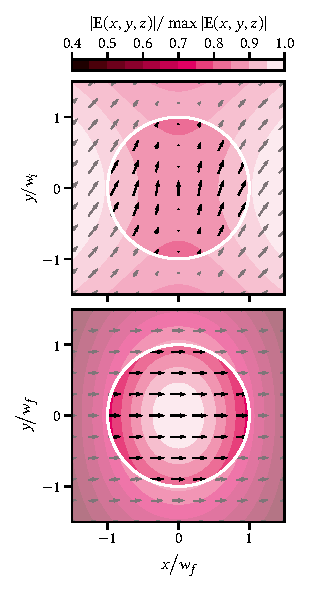
\includegraphics{img/pdf/setup/modes_2d}
    \caption[\imgsource{img/py/setup/single_mode_fiber_coupling.py}]{}
    \label{fig:setup:optics:coupling:modes_2d}
\end{marginfigure}

With the distance of a point in the lens plane from the dipole to good approximation (remember that $d\ll\fob$) given by $r = \sqrt{r_{x}^2 + y^2}$, we can then write the electric field amplitude in the lens plane as
\begin{equation}
    E(x, y) = E_0\e^{\i k \sqrt{r_{x}^2 + y^2}}\sqrt{\frac{1 - \left(\frac{x}{n r_{x}}\right)^2}{r_{x}^2 + y^2}}.
\end{equation}
The normalized intensity $I(x, y) = \abs{E(x, y)}^2$ is shown in the lower panel of \cref{fig:setup:optics:coupling:modes_2d}.
For comparison, the upper panel shows a Gaussian \acrshort{tem}$_{00}$ mode with waist radius $w_0=w\sqrt{2}$ and electric field profile at the focus~\cite{Yariv1989}
\begin{equation}\label{eq:setup:optics:coupling:tem00}
    E(\rho) = E_0\e^{-\flatfrac{\rho^2}{w_0^{2}}},
\end{equation}
with the distance from the beam axis $\rho = \sqrt{x^2 + y^2}$.
The dipole intensity profile is close to circular because the marginal angle $\alpha_\mr{m}=\arcsin(\flatfrac{\mr{\acrshort{na}}}{n})\approx\qty{11}{\degree}$ inside the semiconductor is small and hence the angular dependence of the electric field (\cf \cref{eq:setup:optics:coupling:efield}) is at most $\cos\alpha_\mr{m}\approx 1 - \alpha_{\mr{m}}^2/2 \approx 1$.
Indeed, the fraction of the emitted light cone being collected, the \emph{collection efficiency}, is
\begin{equation}\label{eq:setup:optics:coupling:efficiency:collection}
    \begin{split}
        \eta_{\mr{c}} &= \frac{\iint_{\alpha_{\mr{m}}}\dd{\Omega} I(\alpha)}{\iint\dd{\Omega} I(\alpha)} \\
                      &= \frac{\int_{0}^{\alpha_{\mr{m}}}\dd{\alpha}\sin\alpha\cos^2\alpha}{\int_{0}^{\pi}\dd{\alpha}\sin\alpha\cos^2\alpha} \\
                      &= \frac{1}{2}\left(1 - \left[1 - \left(\frac{\mr{\acrshort{na}}}{n}\right)^2\right]^{\flatfrac{3}{2}}\right)
    \end{split}
\end{equation}
which evaluates to only $\eta_{\mr{c}}\approx\qty{2.8}{\percent}$ for the objective lens's $\mr{\acrshort{na}}=\num{0.7}$.

The light collected and collimated by the objective lens next passes through the ocular lens in the detection arm which focuses it into the \gls{smf}.
The image of the beam on the fiber end face is given by the Fraunhofer diffraction pattern generated by the ocular lens aperture.\sidenote{
    We can safely neglect diffraction effects from the objective lens aperture.
    The Fraunhofer criterion $\flatfrac{b^2}{\lambda}$ with $b$ the aperture diameter is $\approx\qty{30}{\meter}$, implying the ocular lens at a distance of $\sim\qty{1}{\meter}$ is in the near field with many Fresnel zones where diffraction does not yet play a significant role~\cite{Hecht2017}.
}
As the dipole mode clearly falls off much more slowly with distance from the beam axis than the \gls{smf}'s guiding \acrshort{tem}$_{00}$ mode as seen in \cref{fig:setup:optics:coupling:modes_2d}, the coupling efficiency might be limited, thus warranting a more detailed look.
To this end, we approximate the dipole mode as circular -- corresponding to isotropic emission -- so that \cref{eq:setup:optics:coupling:efield} becomes
\begin{equation}\label{eq:setup:optics:coupling:efield:isotropic}
    E(\rho) = E_0\frac{\e^{\i k r_\rho}}{r_\rho}
\end{equation}
with $r_\rho = \sqrt{\rho^2 + \fob^2}$.
Circular symmetry simplifies the Fraunhofer diffraction integral to~\cite{Hecht2017}
\begin{equation}\label{eq:setup:optics:coupling:huygens_fresnel}
    E(q) = \int_{0}^{w}\dd{\rho} \rho J_0(k\rho q/R) E(\rho)
\end{equation}
with $J_0(x)$ the Bessel function of order zero, $q$ the radial coordinate on the image screen, \ie, the fiber end face, and $R$ the distance from the aperture to the screen.
Plugging \cref{eq:setup:optics:coupling:efield:isotropic} into \cref{eq:setup:optics:coupling:huygens_fresnel} and setting $R=\foc$, the focal length of the ocular lens, we obtain
\begin{equation}\label{eq:setup:optics:coupling:huygens_fresnel:evaluated}
    E(q) = E_0\int_{0}^{w}\dd{\rho}\rho J_0(k\rho q/\foc)\frac{\e^{\i k r_\rho}}{r_\rho}.
\end{equation}

The coupling efficiency is then given by the normalized spatial overlap of the light field ($E_{\mr{l}}$, \cref{eq:setup:optics:coupling:efield:isotropic}) and the fiber's guiding mode ($E_{\mr{f}}$, \cref{eq:setup:optics:coupling:tem00}),
\begin{equation}\label{eq:setup:optics:coupling:overlap}
    \begin{split}
        \eta_{\mr{o}} &= \frac{\int\dd{S}\abs{E_{\mr{f}}(x, y)}^2\int\dd{S}\abs{E_{\mr{l}}(x, y)}^2}{\abs{\int\dd{S} E_{\mr{f}}(x, y) E_{\mr{l}}(x, y)}^2} \\
                      &= \frac{\int_{0}^{\infty}\dd{\rho}\rho\abs{E_{\mr{f}}(\rho)}^2\int_{0}^{\infty}\dd{\rho}\rho\abs{E_{\mr{l}}(\rho)}^2}{\abs{\int_{0}^{\infty}\dd{\rho}\rho E_{\mr{f}}(\rho) E_{\mr{l}}(\rho)}^2},
    \end{split}
\end{equation}
where we used the surface element in cylindrical coordinates, $\dd{S}=\rho\dd{\rho}\dd{\phi}$, and already cancelled the angular dependence that is common to all integrals.

\begin{marginfigure}
    \centering
    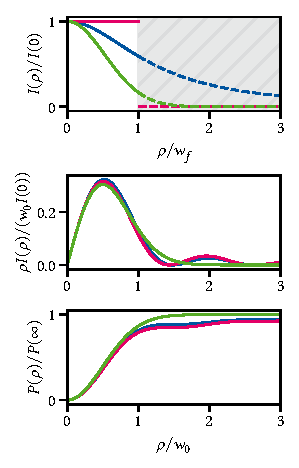
\includegraphics{img/pdf/setup/modes_1d}
    \caption[\imgsource{img/py/setup/single_mode_fiber_coupling.py}]{}
    \label{fig:setup:optics:coupling:modes_1d}
\end{marginfigure}

